In this appendix, evaluation results for several of the synthetic videos are presented. 

In \cref{fig:square_lr_ev} it can be seen how the square moving parallel to two of its edges does not produces spikes for those edges. Only the vertical edge detector spikes in this case, \cref{fig:square_lr_receptive_fields}, and the shapes detector are unable to detect any shape in the visual field, \cref{fig:square_lr_shape}.

In \cref{fig:random_ev} the square and the diamond appear at a certain random location, stay still for about \SIrange{40}{80}{\milli\second} and then disappear and appear in a different location. The edge detectors are spiking only when the shapes change position, \cref{fig:random_receptive_fields}. Consequently, the shapes detectors spike at the same time, but in this case they provide an accurate tracking of the shapes, correctly differentiating between them, \cref{fig:random_shape}.

In \cref{fig:square_diag_ev} the square is moving diagonally from the top left corner to the bottom right one. The direction in which it moves, produces spikes for all edges, as it can be seen in \cref{fig:square_diag_receptive_fields} where both the vertical and horizontal detectors are spiking as expected. The tracking of the square is extremely accurate, as seen in \cref{fig:square_diag_shape}, with some noise due to the square entering the frame. 

%%%%%%%%%%%%%%%%%%%
\begin{figure}[ht]
\centering

\begin{subfigure}{\textwidth}
\centering
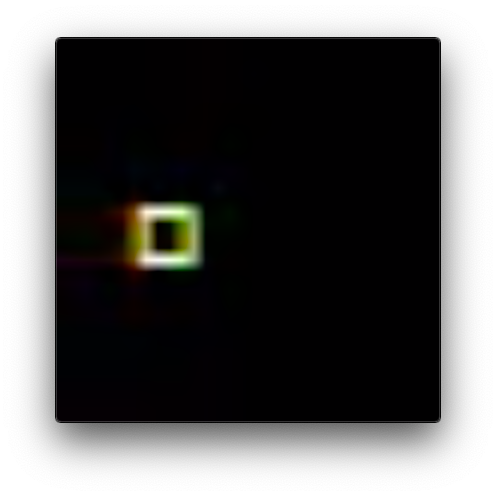
\includegraphics[width=0.3\textwidth]{images/appendix_evaluation/square_lr_spikes.png}
\caption{DVS emulator spikes superimposed over a frame of the video.}
\label{fig:square_lr_spikes}
\end{subfigure}

\begin{subfigure}{\textwidth}
\centering
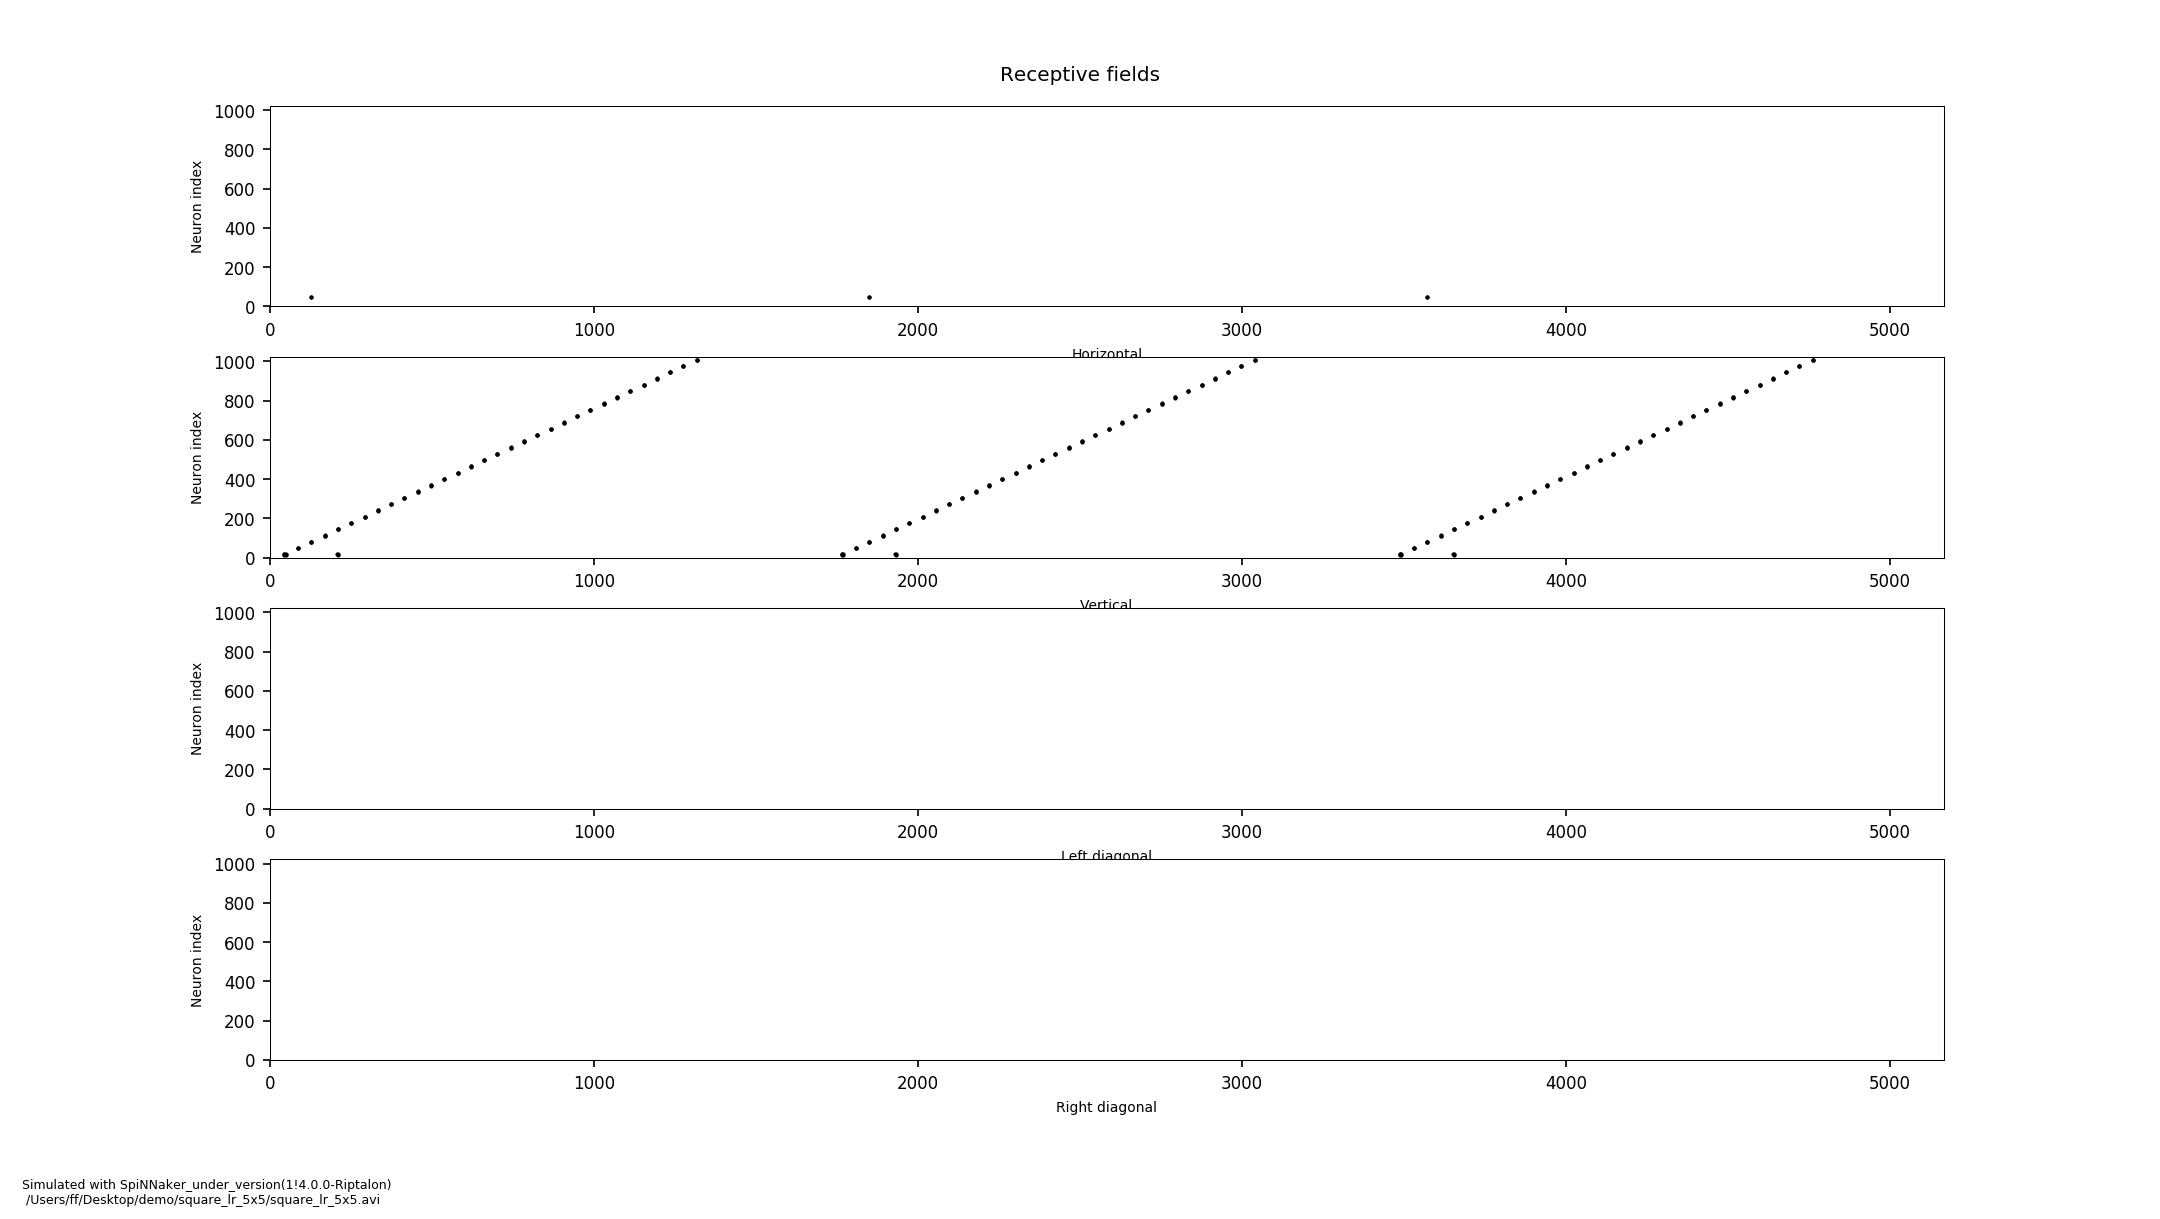
\includegraphics[width=0.75\textwidth]{images/appendix_evaluation/square_lr_receptive_fields.png} 
\caption{Edge detectors.}
\label{fig:square_lr_receptive_fields}
\end{subfigure}

\begin{subfigure}{\textwidth}
\centering
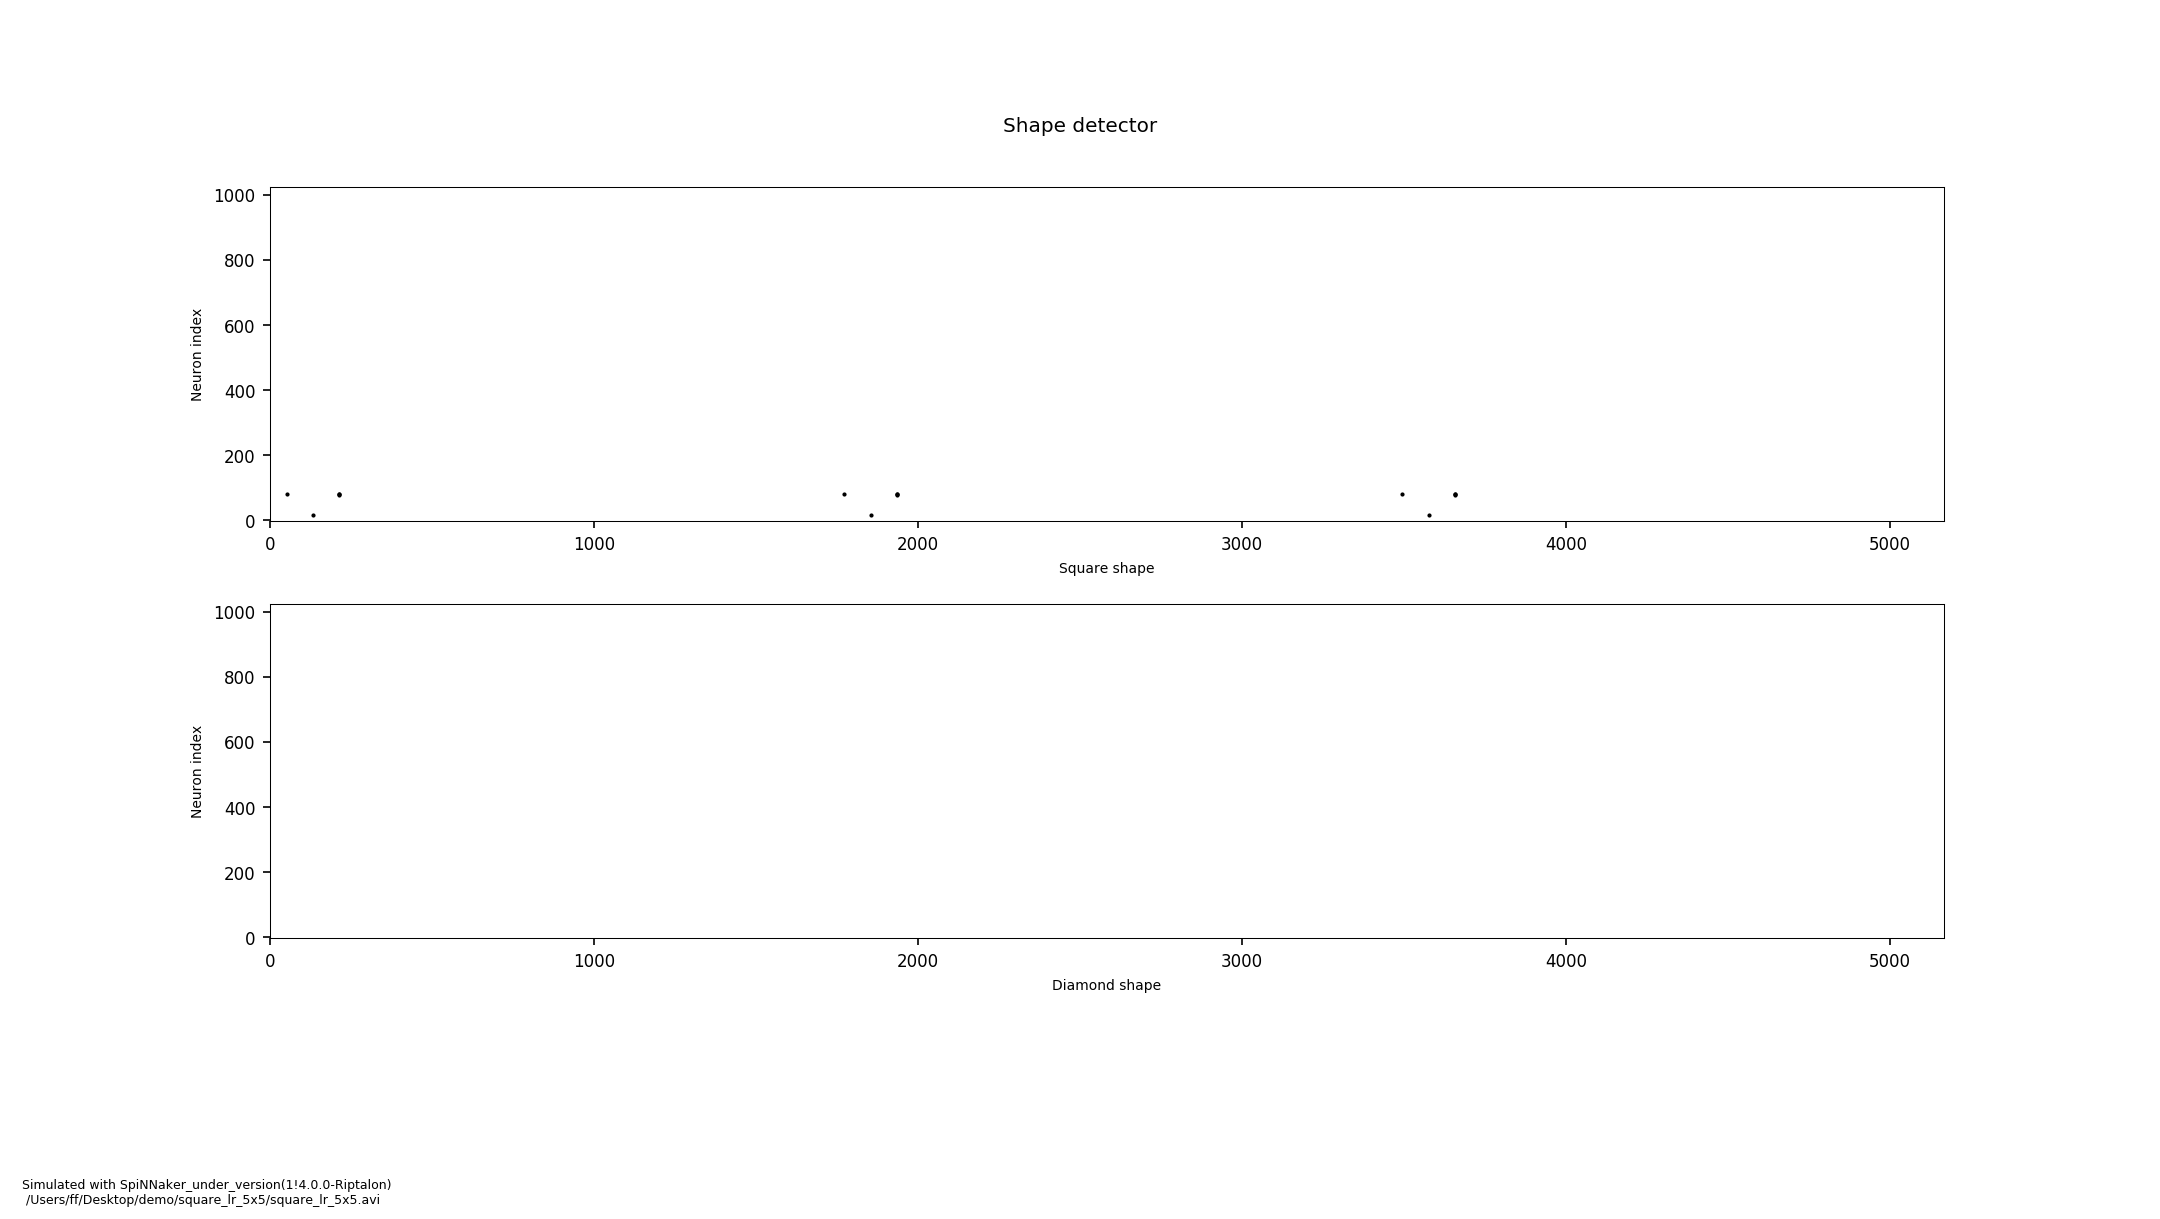
\includegraphics[width=0.75\textwidth]{images/appendix_evaluation/square_lr_shape.png}
\caption{Shapes detector.}
\label{fig:square_lr_shape}
\end{subfigure}

\caption[$5\times 5$ Square Moving Left to Right]{Screenshot and spike trains for the cells populations for a $5\times 5$ square moving from left to right. The video has been generated using a Python script.}
\label{fig:square_lr_ev}
\end{figure}


%%%%%%%%%%%%%%
\begin{figure}[ht]
\centering

\begin{subfigure}{\textwidth}
\centering
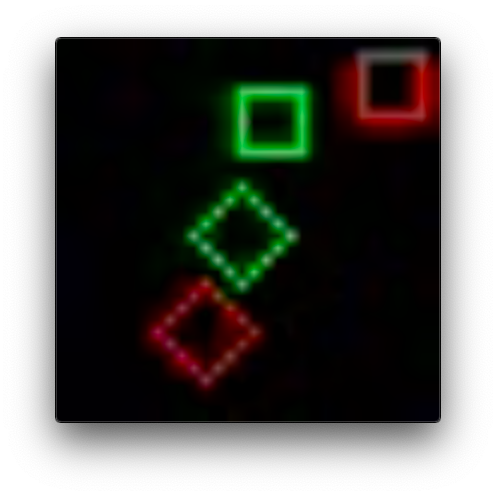
\includegraphics[width=0.3\textwidth]{images/appendix_evaluation/random_spikes.png}
\caption{DVS emulator spikes superimposed over a frame of the video.}
\label{fig:random_spikes}
\end{subfigure}

\begin{subfigure}{\textwidth}
\centering
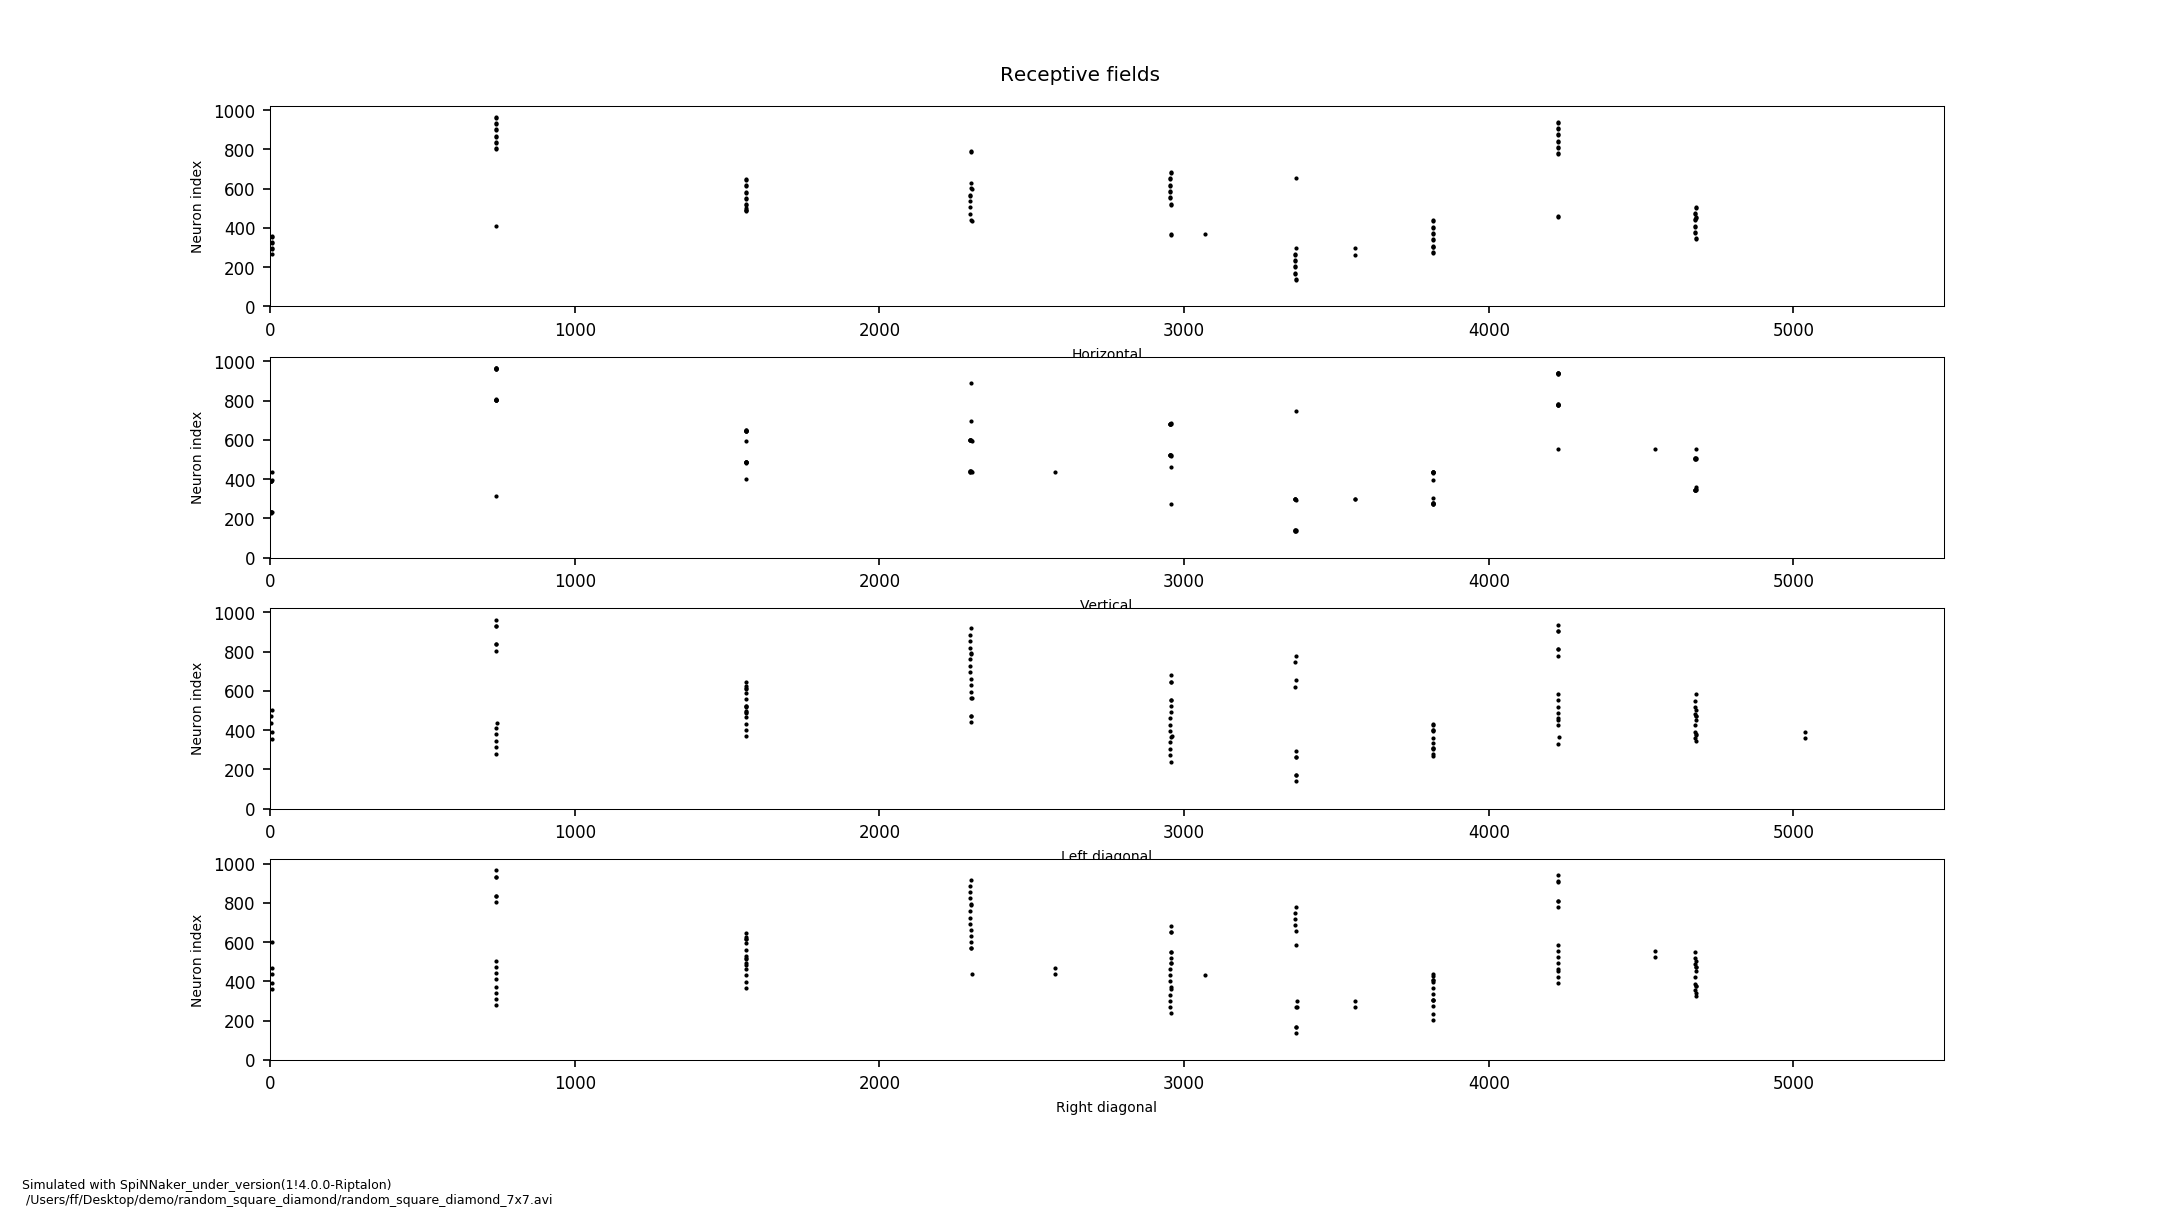
\includegraphics[width=0.75\textwidth]{images/appendix_evaluation/random_receptive_fields.png} 
\caption{Edge detectors.}
\label{fig:random_receptive_fields}
\end{subfigure}

\begin{subfigure}{\textwidth}
\centering
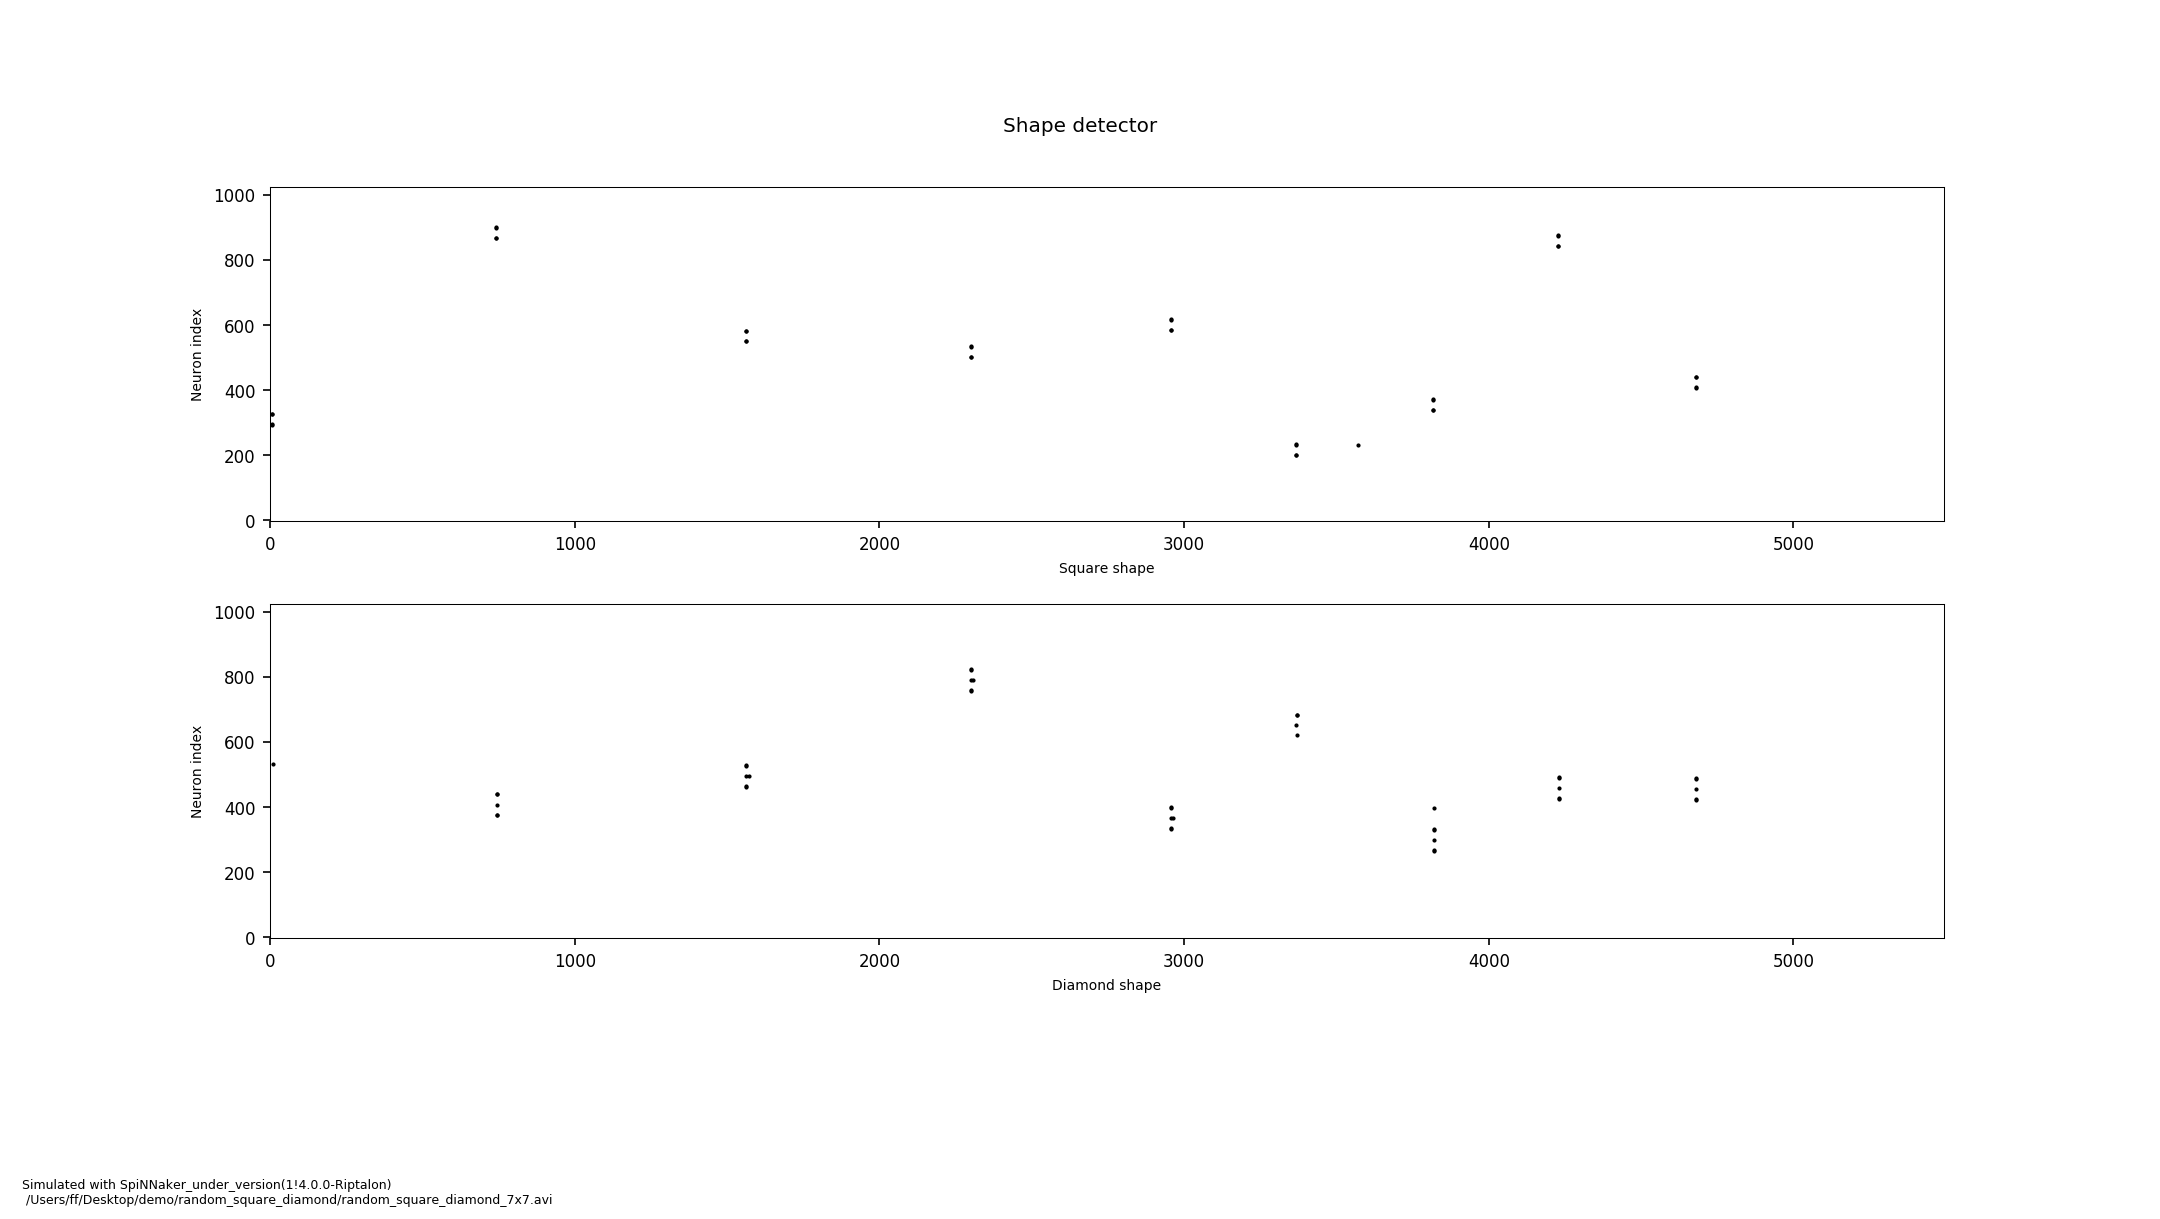
\includegraphics[width=0.75\textwidth]{images/appendix_evaluation/random_shape.png}
\caption{Shapes detector.}
\label{fig:random_shape}
\end{subfigure}

\caption[Square and Diamond Moving Randomly]{Screenshot and spike trains for the cells populations for a $5\times 5$ square and a $5\times 5$ diamond appearing at random locations. The video has been generated using a Python script.}
\label{fig:random_ev}
\end{figure}


%%%%%%%%%%%%%%%%%%%
\begin{figure}[ht]
\centering

\begin{subfigure}{\textwidth}
\centering
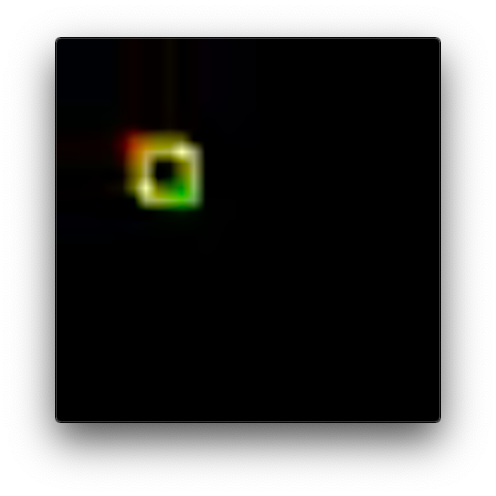
\includegraphics[width=0.3\textwidth]{images/appendix_evaluation/square_diag_spikes.png}
\caption{DVS emulator spikes superimposed over a frame of the video.}
\label{fig:square_diag_spikes}
\end{subfigure}

\begin{subfigure}{\textwidth}
\centering
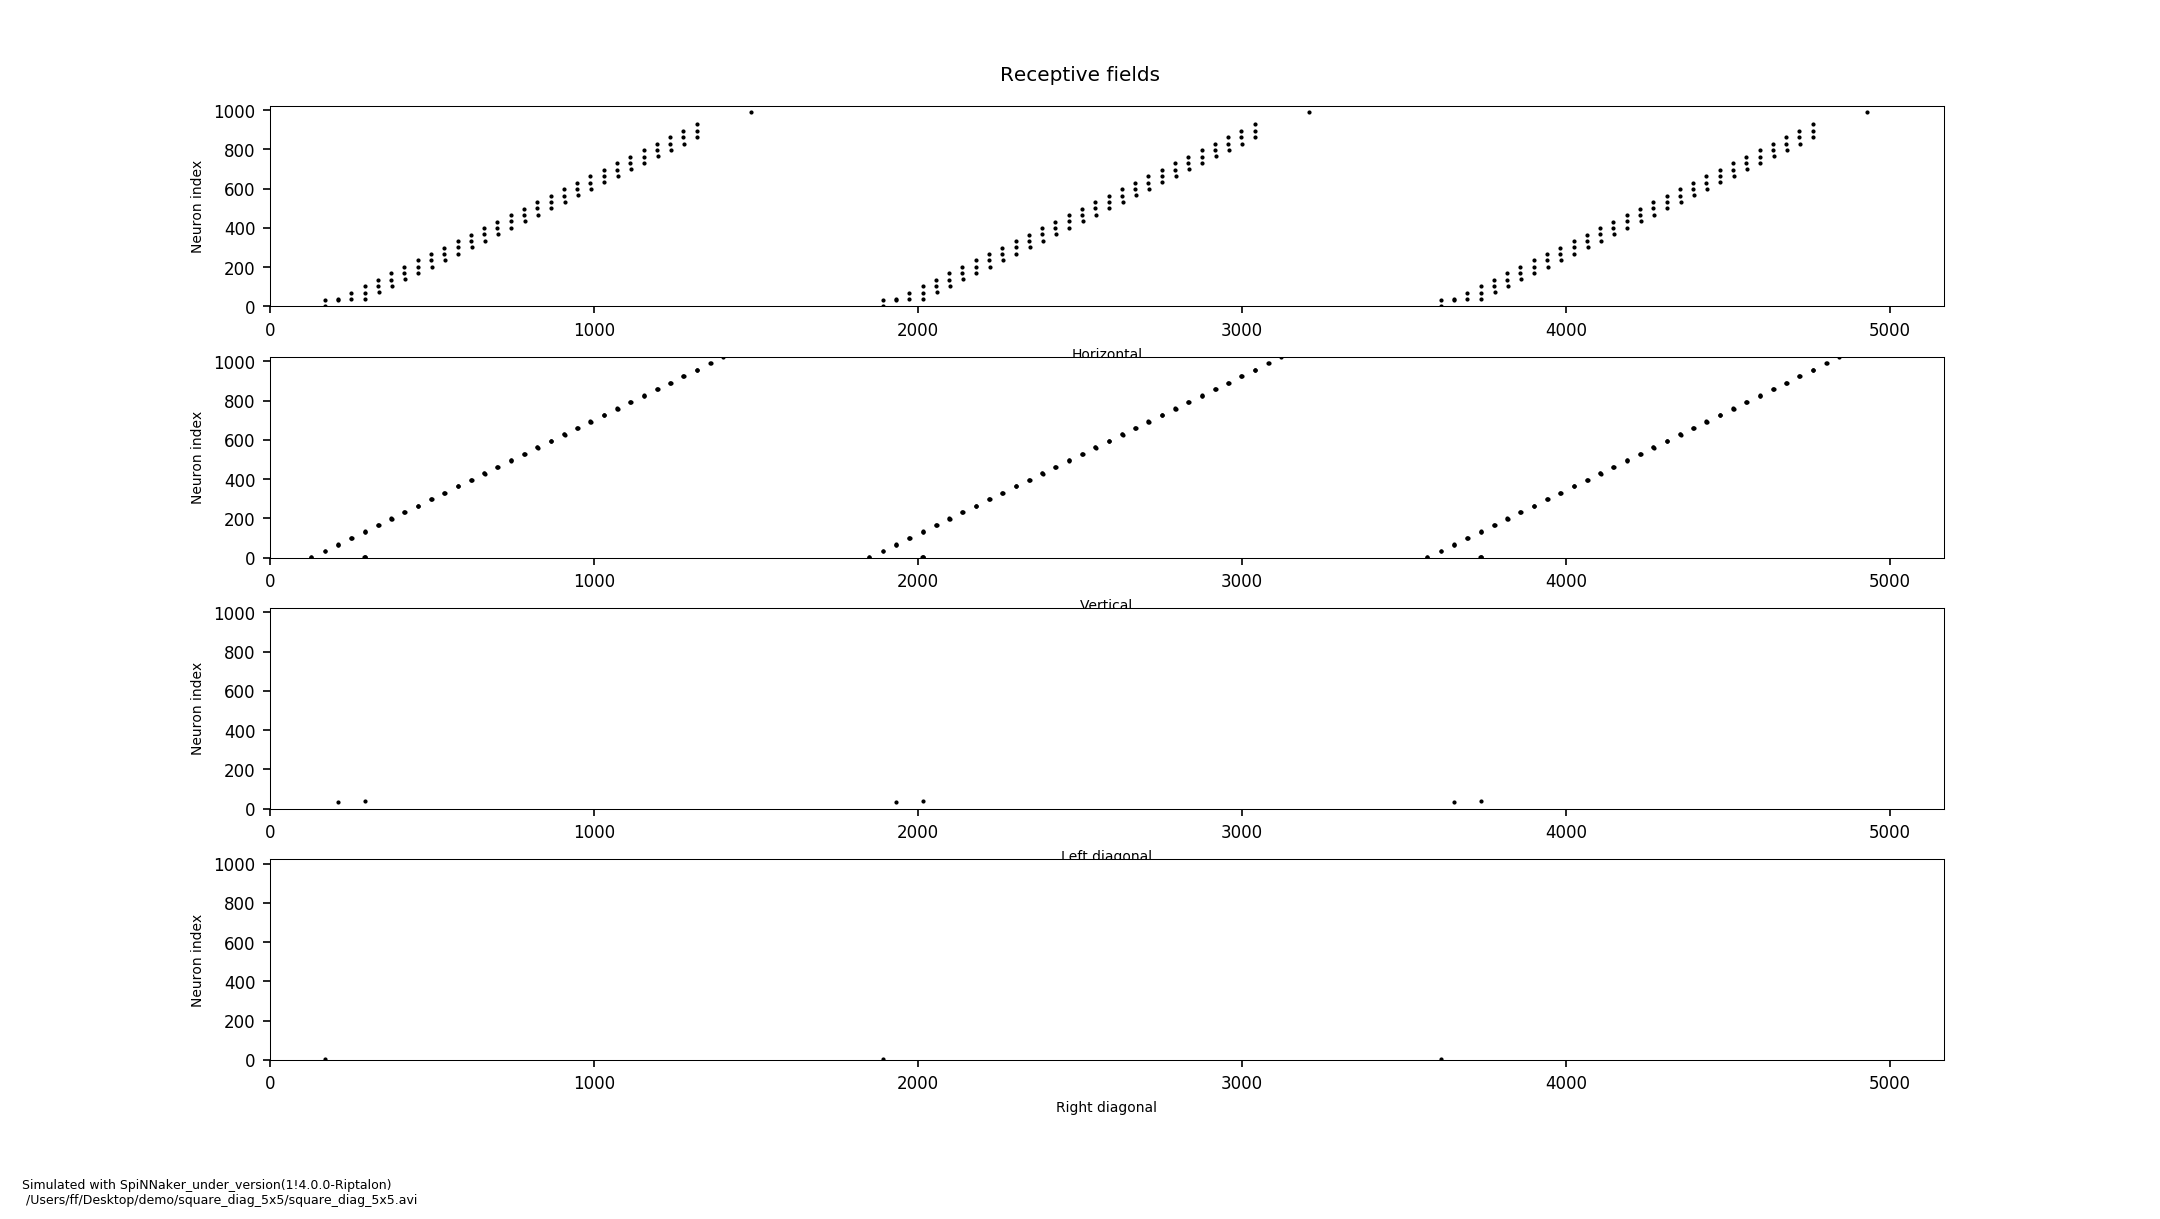
\includegraphics[width=0.75\textwidth]{images/appendix_evaluation/square_diag_receptive_fields.png} 
\caption{Edge detectors.}
\label{fig:square_diag_receptive_fields}
\end{subfigure}

\begin{subfigure}{\textwidth}
\centering
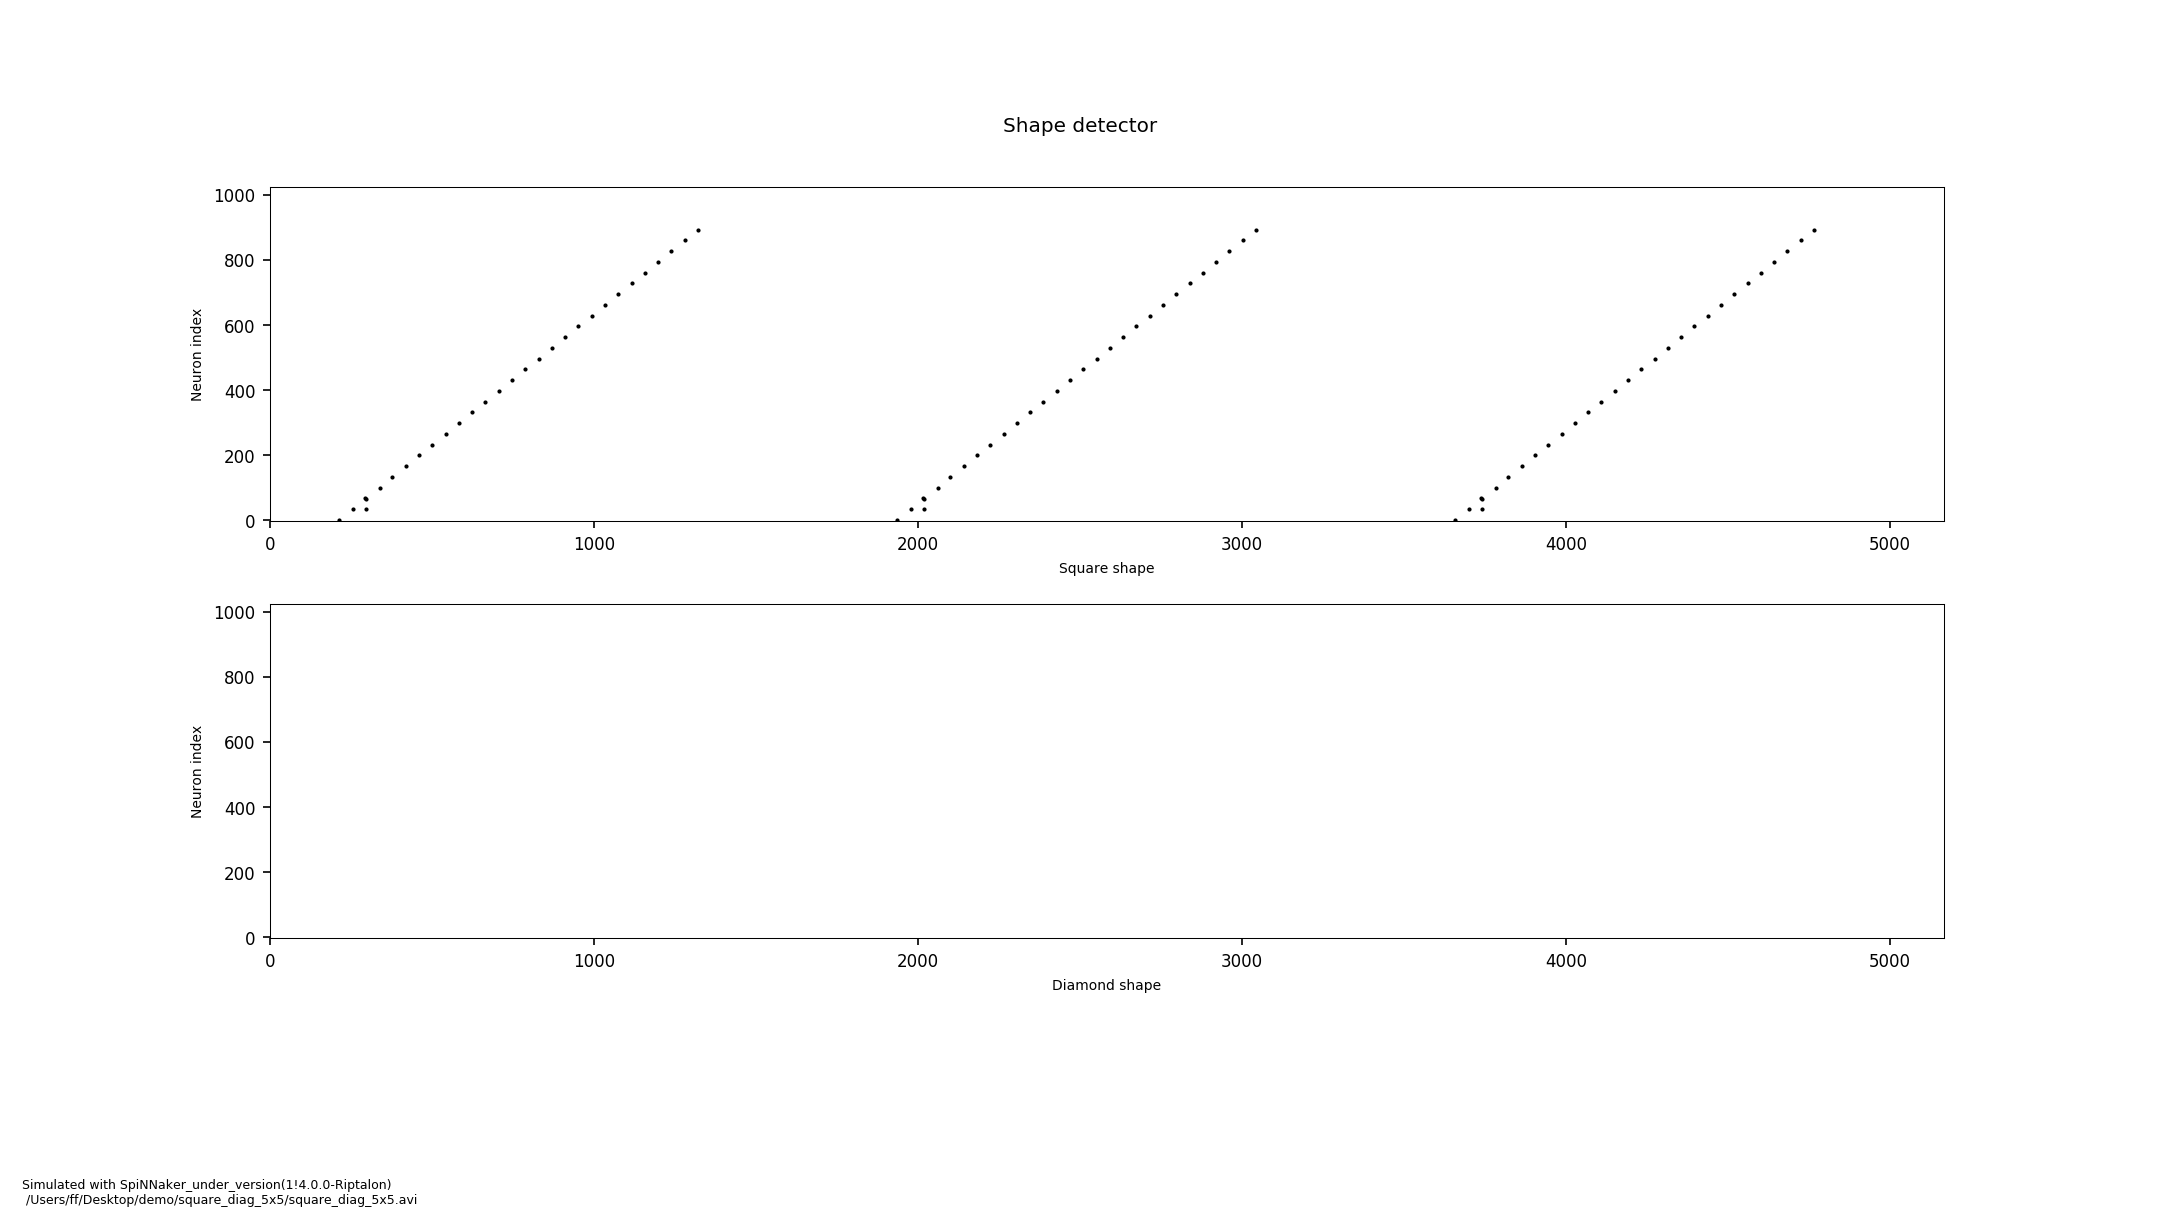
\includegraphics[width=0.75\textwidth]{images/appendix_evaluation/square_diag_shape.png}
\caption{Shapes detector.}
\label{fig:square_diag_shape}
\end{subfigure}

\caption[$5\times 5$ Square Moving Diagonally]{Screenshot and spike trains for the cells populations for a $5\times 5$ square moving from the top left corner to the bottom right corner. The video has been generated using a Python script.}
\label{fig:square_diag_ev}
\end{figure}
